\documentclass[11pt]{article}
% Self-contained: no \input, no external .bib, no image files (plots are drawn by pgfplots
% from inline data).  Compile with pdflatex/tectonic.
\usepackage[margin=1in]{geometry}
\usepackage{amsmath,amssymb,amsthm,mathtools}
\usepackage{booktabs}
\usepackage{enumitem}
\usepackage[title,titletoc]{appendix}
\usepackage{array,longtable}
\usepackage{microtype}
\usepackage{pgfplots}
\pgfplotsset{compat=1.17}
\usepackage{url}
\usepackage[colorlinks=true,linkcolor=blue!50!black,citecolor=green!40!black,urlcolor=blue!60!black]{hyperref}

\newcommand{\ad}{\operatorname{ad}}
\newcommand{\Ad}{\operatorname{Ad}}
\newcommand{\norm}[1]{\lVert #1\rVert}
\newcommand{\abs}[1]{\lvert #1\rvert}
\newcommand{\Q}{\mathbb{Q}}
\newcommand{\Qc}{\mathbb{Q}(2^{1/3})}
\newcommand{\Lie}{\mathcal{L}}
\newcommand{\C}[1]{C_{\mathsf{#1}}}
\newcommand{\lb}[1]{[#1]}
\newcommand{\dd}{\,\mathrm{d}}
\newcommand{\codeus}{\textunderscore\allowbreak}
\newcommand{\code}[1]{{\ttfamily\let\_\codeus\hyphenchar\font=-1 #1}}

\theoremstyle{plain}
\newtheorem{theorem}{Theorem}
\renewcommand{\thetheorem}{\Alph{theorem}}
\newtheorem{proposition}{Proposition}
\newtheorem{lemma}{Lemma}
\newtheorem{corollary}{Corollary}
\theoremstyle{definition}
\newtheorem{definition}{Definition}
\theoremstyle{remark}
\newtheorem{remark}{Remark}

\title{Tightening the rigorous error bound of the fourth-order Suzuki--Trotter formula}
\author{Areg Gevorgyan\\ University of Maryland, College Park\\ \href{mailto:areg@umd.edu}{\texttt{areg@umd.edu}}}
\date{Caltech Mathathon, Problem \#109 --- November 2026\\[0.6em]
\small Repository: \url{https://github.com/AregGevorgyan/mathathon}}

\begin{document}
\maketitle

\begin{abstract}
For $H=A+B$ with bounded anti-Hermitian $A,B$ and the fourth-order Suzuki product formula $S_4(t)$,
the standard rigorous bound of Childs, Su, Tran, Wiebe and Zhu~\cite{Childs2021} is
$\norm{S_4(t)-e^{tH}}\le t^5\sum_w\gamma_w\norm{C_w}$ over eight nested commutators $C_w$, with
$\sum_w\gamma_w=0.0875$. We (i) compute the leading local error term exactly,
$\log S_4(t)=tH+t^5E_5+O(t^7)$, with coordinates in $\Qc$; (ii) prove all-$t$ bounds whose $t^5$
constant is exactly this leading term ($\sum\abs{e_w}=0.0029982$, $29\times$ below $0.0875$) with explicit
$t^6,t^7$ remainders, and a single-term bound ($0.01367$) that is coefficientwise below~\cite{Childs2021};
(iii) make the known non-accumulation of the $[H,\cdot\,]$ part of the error fully explicit for $S_4$, so that
the error grows with total time $T$ only through $\lb Z=0.000891$; and (iv) prove, by linear-programming
duality with six explicit matrix pairs and exact rational arithmetic, that no bound of this commutator
form can have leading constant below $0.0029981499$, so ours is optimal to relative $3\cdot10^{-6}$.
The analytic argument is formalised in Lean~4/Mathlib without \texttt{sorry}, the leading term is
certified by Lean's kernel, and an independent derivation uses the Alkahest computer-algebra system. On
transverse-field Ising chains the guaranteed step count is within $2.2\%$ ($n=8$, $T=128$) and $0.37\%$
($n=1000$) of the true requirement, against a factor $\approx4.2$ for~\cite{Childs2021}.
\end{abstract}

\tableofcontents

%======================================================================
\section{Problem, motivation, and prior work}\label{sec:intro}

\paragraph{Problem.} Product formulas approximate $e^{t(A+B)}$ by products of $e^{sA}$ and $e^{sB}$.
They are the simplest and most widely used algorithms for Hamiltonian simulation on quantum computers,
and the number of gates scales with the number of time steps $r$ needed to reach a target error
$\varepsilon$. A rigorous bound on the error therefore translates directly into a resource estimate.
We aim to find a rigorous finite-step bound on the fourth-order Suzuki formula with
a strictly smaller prefactor than Childs et al.~\cite{Childs2021}, obtained from the exact leading
$t^5$ term plus a controlled remainder; a comparison with the bound of Schubert and
Mendl~\cite{SchubertMendl2023} and with the true error on the transverse-field Ising model; and a
discussion relative to the local-error representation of Descombes and
Thalhammer~\cite{DescombesThalhammer2010}.

\paragraph{Known limitation.} Commutator-scaling bounds~\cite{Childs2021} expand the error in nested
commutators and apply the triangle inequality monomial by monomial. This captures the correct scaling
but loses constant factors: for fourth-order formulas the bounds overestimate the true error by about
three orders of magnitude, as Schubert and Mendl observe numerically~\cite{SchubertMendl2023}, who
attribute the gap to cancellations discarded by the triangle inequality. Multiplying a one-step bound by
$r$ loses a further factor, because errors of consecutive steps partly cancel; for first-order Trotter
this was made rigorous by Layden~\cite{Layden2022}.

\paragraph{Prior work in brief.} Commutator-scaling bounds originate
in~\cite{ChildsSu2019,Childs2021}, building on the local-error representation
of~\cite{DescombesThalhammer2010}; Schubert and Mendl~\cite{SchubertMendl2023} generalise them with
smaller prefactors. The leading local error of splitting methods is a Lie element~\cite{AuzingerHerfort2014},
and leading-error coefficients of Suzuki-type schemes have been tabulated numerically to rank
schemes~\cite{McLachlan1995,Omelyan2002,BarthelZhang2020,Ostmeyer2023}. Error cancellation across steps
was proved for first-order formulas~\cite{Tran2020,Layden2022} and recently characterised for general
order: the error component of the form $[H,\cdot\,]$ does not accumulate~\cite{ChenYH2025,ChenXuYuanZhao2026}.
Section~\ref{sec:prior} discusses these and other recent directions in detail.

\paragraph{Contributions to literature.} We keep the commutator-norm form of~\cite{Childs2021} (so all bounds are
operator-independent and directly comparable) but (a) compute the leading term exactly, (b) expand the
remainder so that every surviving exponential is an outer unitary conjugation and all cancellations
happen \emph{before} norms are taken, (c) telescope the $[H,\cdot\,]$ part of the error over steps, and
(d) prove that the resulting leading constant cannot be improved within this form. To our
knowledge, new are: the exact closed form of the $S_4$ leading term in $\Qc$ (previously known
numerically~\cite{BarthelZhang2020}) used as the constant of a rigorous all-$t$ bound; the
cancellation-preserving remainder (Lemma~\ref{lem:taylor}) with explicit constants; fully explicit
many-step constants for $S_4$ realising the known $[H,\cdot\,]$ mechanism; the optimality proof
(Theorem~\ref{thm:E}); and a machine-checked formalisation of the analytic argument.
Section~\ref{sec:rigorous} contains only rigorous statements; Section~\ref{sec:numerics} contains
numerical evidence, which is clearly marked as such.

%======================================================================
\section{Notation and setting}\label{sec:notation}

$A,B$ are bounded anti-Hermitian operators, equivalently $e^{tA}=e^{-itA_{\rm phys}}$ with Hermitian
$A_{\rm phys}=iA$. We write
\[
H=A+B,\qquad U(t)=e^{tH},
\]
and $\norm\cdot$ for the operator norm. Unitary conjugation preserves norms, and nested-commutator
norms are unchanged by the factor $i$. More generally, every analytic statement holds in a real Banach
algebra in which every generator $a$ satisfies
\[
\norm{e^{sa}}\le1\qquad\text{for all real }s.
\]

\paragraph{The formula.} The second- and fourth-order Suzuki formulas are
\[
S_2(t)=e^{tA/2}e^{tB}e^{tA/2},\qquad
S_4(t)=S_2(pt)^2S_2(qt)S_2(pt)^2,\qquad p=\frac1{4-4^{1/3}},\quad q=1-4p .
\]
Merging adjacent $A$-factors gives eleven stages (product taken left to right),
\[
S_4(t)=\prod_{j=1}^{11}e^{tc_jX_j},\qquad
(c_j)=\bigl(\tfrac p2,\,p,\,p,\,p,\,\tfrac{1-3p}2,\,q,\,\tfrac{1-3p}2,\,p,\,p,\,p,\,\tfrac p2\bigr),
\]
with $X_j$ alternating $A,B,\dots,A$. With $\varpi=2^{1/3}$,
\[
p=\tfrac4{15}+\tfrac1{30}\varpi+\tfrac1{15}\varpi^2\in\Qc,
\]
so all exact quantities below lie in $\Qc$.

\paragraph{Commutators.} $\Lie_d$ is the degree-$d$ part of the free Lie algebra on $\{A,B\}$
($\dim\Lie_5=6$, $\dim\Lie_6=9$, $\dim\Lie_7=18$). For a word $w=x_1\cdots x_k$ over
$\{\mathsf A,\mathsf B\}$, the right-nested commutators used in~\cite{Childs2021} are
\[
\C w=[X_{x_1},[X_{x_2},\dots,[X_{x_k},[A,B]]\cdots]],\qquad\text{e.g. }\C{BAB}=[B,[A,[B,[A,B]]]].
\]
They span $\Lie_{k+2}$ but are linearly dependent. Since $[[B,A],[A,B]]=0$, the Jacobi identity gives
\[
\C{w\mathsf{BA}}=\C{w\mathsf{AB}},
\]
so in degree~5 the eight $\C w$ are six distinct operators. We write
\[
\ad_XY=[X,Y],\qquad \Ad_{e^{sX}}Y=e^{sX}Ye^{-sX}.
\]

\paragraph{Hall and Lyndon bases.} The free Lie algebra $\Lie$ on $\{A,B\}$ consists of all linear
combinations of iterated brackets of $A$ and $B$, subject only to antisymmetry and the Jacobi identity.
Its degree-$d$ part has dimension given by Witt's formula,
\[
\dim\Lie_d=\frac1d\sum_{e\mid d}\mu(e)\,2^{d/e}\qquad(\dim\Lie_4=3,\ \dim\Lie_5=6,\ \dim\Lie_6=9,\ \dim\Lie_7=18),
\]
with $\mu$ the M\"obius function. Since spanning sets of brackets are redundant, one fixes a basis to
make coefficients unique. A \emph{Hall basis}~\cite{Hall1950,Reutenauer1993} is a set of brackets
built recursively from the letters together with a total order on brackets: a bracket $[t',t'']$ of
two admitted brackets is admitted when $t'<t''$ and, if $t'=[x,y]$ is itself a bracket, $y\le t''$
(one common convention). The admitted brackets of degree $d$ form a basis of $\Lie_d$. A \emph{Lyndon word} is a nonempty word over $\mathsf A<\mathsf B$
that is lexicographically smaller than each of its proper suffixes (e.g.\ $\mathsf{AAAB}$, $\mathsf{AABB}$,
$\mathsf{ABBB}$ in length~4). Its \emph{standard bracketing} is defined by $b(\mathsf A)=A$, $b(\mathsf B)=B$
and $b(w)=[b(u),b(v)]$, where $w=uv$ and $v$ is the longest proper suffix of $w$ that is a Lyndon word.
The bracketings of the Lyndon words of length $d$ form the \emph{Lyndon basis} of
$\Lie_d$~\cite{Reutenauer1993}, a particular Hall basis. In degree~4 it is
\[
[A,[A,[A,B]]],\qquad [A,[[A,B],B]],\qquad [[[A,B],B],B].
\]
Proposition~\ref{prop:leading} states $E_5$ in a Hall basis $C_1,\dots,C_6$ of $\Lie_5$, where its six
coordinates are unique. The right-nested commutators $\C w$ above span $\Lie_d$ but are not a basis;
they are used for the bounds because they are the family of~\cite{Childs2021}.

\paragraph{Universal constants.} A Lie polynomial $P\in\Lie_d$ is written exactly as
$P=\sum_wx_w\C w$ with $x_w\in\Qc$, using an $\ell^1$-minimal representation. We write
\[
\lb P=\sum_w\abs{x_w},\qquad\text{so that}\qquad \norm P\le\sum_w\abs{x_w}\,\norm{\C w}.
\] Every bound below carries individual coefficients per
commutator (Appendix~\ref{app:tables}); a ``constant'' quoted as a single number is the sum of those
coefficients, i.e.\ the bound with all $\norm{\C w}=1$. Decimals are rigorous upper bounds unless
marked $\approx$.

%======================================================================
\section{Rigorous results}\label{sec:rigorous}

\subsection{The exact leading term}

\begin{proposition}\label{prop:leading}
In the free Lie algebra,
\[
\log S_4(t)=t(A+B)+t^5E_5+O(t^7),\qquad E_5=\sum_{i=1}^6c_iC_i,
\]
in the Hall basis
\begin{gather*}
C_1=[A,[A,[A,[A,B]]]],\quad C_2=[B,[A,[A,[A,B]]]],\quad C_3=[B,[B,[A,[A,B]]]],\\
C_4=[B,[B,[B,[A,B]]]],\quad C_5=[[A,B],[A,[A,B]]],\quad C_6=[[A,B],[B,[A,B]]]
\end{gather*}
and
\[
\begin{aligned}
c_1&=-\tfrac{169}{1350000}-\tfrac{1}{28125}\varpi-\tfrac{2437}{43200000}\varpi^2,&
c_2&=-\tfrac{169}{337500}-\tfrac{4}{28125}\varpi-\tfrac{2437}{10800000}\varpi^2,\\
c_3&=-\tfrac{551}{900000}-\tfrac{451}{2700000}\varpi-\tfrac{371}{1350000}\varpi^2,&
c_4&=-\tfrac{301}{1350000}-\tfrac{67}{1350000}\varpi-\tfrac{59}{600000}\varpi^2,\\
c_5&=-\tfrac{301}{900000}-\tfrac{67}{900000}\varpi-\tfrac{59}{400000}\varpi^2,&
c_6&=-\tfrac{17}{150000}+\tfrac{49}{1350000}\varpi-\tfrac{109}{2700000}\varpi^2 .
\end{aligned}
\]
Over right-nested commutators (Table~\ref{tab:E5}),
\[
E_5=\sum_we_w\C w,\qquad \lb{E_5}=\sum_w\abs{e_w}\approx0.0029982 .
\]
\end{proposition}

\begin{proof}[Proof (computer-assisted, exact)]
Multiply the eleven exponentials in the algebra of noncommutative polynomials truncated at degree~7
with coefficients in $\Qc$, and take the truncated logarithm. The degree-2, 3, 4 and 6 parts vanish,
the degree-1 part is $A+B$, and the degree-5 part solves an overdetermined linear system over all 32
words consistently in the Hall basis, which certifies that it is a Lie element with the stated
coordinates. Three independent checks are in \S\ref{sec:verification}.
\end{proof}

Since
\[
\norm{S_4(t)-U(t)}=t^5\norm{E_5}+O(t^6),
\]
the constant $\norm{E_5}$ is the optimal $t^5$ prefactor for any given $H$.

\subsection{An error representation that keeps cancellations}

The remainder is controlled by one variation-of-constants (Duhamel) identity, Lemma~\ref{lem:voc},
iterated along the stage structure that the Suzuki recursion produces (Lemmas~\ref{lem:tele} and~\ref{lem:taylor}). This is the Descombes--Thalhammer
representation~\cite{DescombesThalhammer2010} specialised to bounded operators, with a different
expansion of the integrand (\S\ref{sec:prior}). Split the stages as $S_4=LR$ with $L$ the first $m$ stages and $R$ the rest.

\begin{lemma}[variation of constants]\label{lem:voc}
Let $T(\tau)=L^{-1}L'+R'R^{-1}-L^{-1}HL$. Then
\[
S_4'-HS_4=L\,T\,R\qquad\text{and}\qquad \norm{S_4(t)-U(t)}\le\int_0^t\norm{T(\tau)}\dd\tau .
\]
\end{lemma}

\begin{lemma}[telescoping into chains]\label{lem:tele}
For generators $a_1,\dots,a_n$ and a terminal element $Z_0$ define the \emph{chain}
\[
V(\tau)=a_1+\Ad_{e^{\tau a_1}}\Bigl(a_2+\Ad_{e^{\tau a_2}}\bigl(\cdots(a_n+\Ad_{e^{\tau a_n}}Z_0)\bigr)\Bigr).
\]
Then $T=V_{\rm right}-V_{\rm left}$, where the right chain has the stages $m+1,\dots,11$ (generators
$c_jX_j$) and terminal $0$, and the left chain has the stages $m,\dots,1$ with negated generators and
terminal $H$. For $m=0$, $S_4'=V\,S_4$.
\end{lemma}

\begin{lemma}[Taylor expansion from the right]\label{lem:taylor}
Let $c_r$ be the Taylor coefficients of a chain, given by the exact recursion
\[
c(a{:}L,r)=[r{=}0]\,a+\sum_{k\le r}\frac{\ad_a^{r-k}c(L,k)}{(r-k)!}.
\]
For $K\ge1$ and $\tau\ge0$,
\[
\Bigl\lVert V(\tau)-\sum_{r<K}\tau^rc_r\Bigr\rVert\le\tau^K\sum_{s}\int_0^1\norm{P_s(u)}\dd u,
\]
\[
P_s(u)=\sum_{j<K}\frac{(1-u)^{K-j-1}}{(K-j-1)!}\,\ad_{a_s}^{K-j}c(\mathrm{tail}_s,j),
\]
where $s$ runs over the items and $\mathrm{tail}_s$ is the chain after item $s$.
\end{lemma}

Every $\ad_{a_s}^{K-j}c(\mathrm{tail}_s,j)$ is an exact Lie polynomial, normed only after all
cancellations inside the tail; all conjugations have dropped out of the norm; and different orders
$K-j$ of the same item are normed \emph{together} (``grouping across orders''). Bounding orders
separately (the triangle inequality in $j$) loses a factor $1.8$--$2.6$ in the universal constants.
Proofs are in Appendix~\ref{app:proofs}; all three lemmas are formalised in Lean
(\S\ref{sec:verification}). Combining them,
\begin{equation}\tag{$\star$}\label{eq:star}
\norm{S_4(t)-U(t)}\le\sum_{n=4}^{K-1}\frac{t^{n+1}}{n+1}\norm{t_n}+\frac{t^{K+1}}{K+1}\,\Gamma_{K+1},
\end{equation}
where $t_n$ are the Taylor coefficients of $T$, with
\[
t_n=0\ (n<4),\qquad t_4=5E_5,
\]
and $\Gamma_{K+1}$ is the sum of the Lemma~\ref{lem:taylor} integrals of both chains. Writing every grouped polynomial over right-nested
commutators and applying the triangle inequality under the integral gives operator-independent
constants; the integrals $\int_0^1\abs{c_{s,w}(u)}\dd u$ are bounded by rational interval arithmetic.
Because the $\C w$ are dependent, the representation of each grouped polynomial may be shifted by the
kernel
\[
\Bigl\{(y_w):\ \sum_wy_w\C w=0\Bigr\};
\]
we choose the shifts of all orders jointly by a linear program and then
round them to rationals, so every identity stays exact (``joint representations'').

\subsection{Single-step theorems}

\begin{theorem}[single $t^5$ term]\label{thm:A}
For all $t\ge0$ ($K=4$, $m=0$):
\begin{multline*}
\norm{S_4(t)-e^{tH}}\le t^5\bigl(0.000675\norm{\C{AAA}}+0.002040\norm{\C{AAB}}+0.001668\norm{\C{ABB}}\\
+0.001424\norm{\C{BAA}}+0.004279\norm{\C{BAB}}+0.003583\norm{\C{BBB}}\bigr).
\end{multline*}
The coefficients sum to $0.01367$, against $0.0875$ for~\cite[Prop.~J.1]{Childs2021}, and each is below
the corresponding coefficient there, so the bound improves on~\cite{Childs2021} for every $H$.
\end{theorem}

\begin{theorem}[exact leading term, $t^6$ remainder]\label{thm:B}
For all $t\ge0$ ($K=5$, $m=3$),
\[
\norm{S_4(t)-e^{tH}}\le t^5\sum_w\abs{e_w}\norm{\C w}+t^6\sum_wd_w\norm{\C w},\qquad
\textstyle\sum_w\abs{e_w}\approx0.0029982,\quad\sum_wd_w\le0.002943 .
\]
\end{theorem}

\begin{theorem}[exact $t^5$ and $t^6$ terms, $t^7$ remainder]\label{thm:C}
For all $t\ge0$ ($K=6$, $m=2$),
\[
\norm{S_4(t)-e^{tH}}\le t^5\sum_w\abs{e_w}\norm{\C w}+t^6\sum_wf_w\norm{\C w}+t^7\sum_wh_w\norm{\C w},
\]
with $\sum_wf_w\approx0.0004993$ exact and $\sum_wh_w\le0.0006659$.
\end{theorem}

For $t\lesssim1$ Theorem~C is the strongest: its $t^5$ constant is the exact leading term, and its
$t^6$, $t^7$ constants are about $175\times$ and $130\times$ smaller than the entire constant
of~\cite{Childs2021}. Evaluated with the norms of a specific $H$, \eqref{eq:star} is asymptotically exact
(its ratio to the true error tends to~1 as $t\to0$).

\subsection{Many-step theorems: the \texorpdfstring{$[H,\cdot\,]$}{[H,.]} part telescopes}

For total time $T$ and $r$ steps let
\[
\delta=T/r,\qquad M=U(-\delta)S_4(\delta)-1,\qquad\text{so that}\qquad S_4(\delta)-U(\delta)=U(\delta)M,
\]
and split the leading term as
\[
E_5=[H,Y]+Z,\qquad Y\in\Lie_4 .
\]

\begin{theorem}[many steps]\label{thm:D}
For all $T>0$, $r\ge1$, $\delta=T/r$, and any $Y$, with $b$ the bound of Theorem~C,
\[
\begin{aligned}
\norm{S_4(\delta)^r-e^{TH}}\le{}&T\delta^4\norm Z+2\delta^4\norm Y
+T\delta^6\Bigl(\tfrac{\norm{\ad_H^3Y}}{24}+\tfrac{\norm{\ad_H^2E_5}}8+\tfrac{\hat\Gamma_7}7\Bigr)
+T\delta^4\hat\Gamma_5\,\tfrac{b(\delta)}5+\tfrac{T^2b(\delta)^2}{2\delta^2},
\end{aligned}
\]
where $\hat\Gamma_K$ are the Lemma~\ref{lem:taylor} constants of $\hat S(\tau)=e^{-\tau H}S_4(\tau)$.
\end{theorem}

The proof (Appendix~\ref{app:proofs}) has three steps.
\begin{enumerate}[leftmargin=*]
\item Telescoping over steps:
\[
S^r-U^r=\sum_jU^{r-1-j}(S-U)U^j+O\bigl(\norm{S-U}^2r^2\bigr).
\]
\item Lemma~\ref{lem:taylor} applied to $\hat S$, whose Taylor coefficients are
$\hat c_0=\dots=\hat c_3=0$, $\hat c_4=5E_5$, $\hat c_5=-3[H,E_5]$, gives
\[
\norm{M-\delta^5\Ad_{U(-\delta/2)}E_5}\le\rho(\delta).
\]
\item Midpoint telescoping: since $\Ad_{U(-s)}[H,Y]=-\tfrac{d}{ds}\Ad_{U(-s)}Y$,
\[
\Bigl\lVert\sum_j\delta\,\Ad_{U(-(j+\frac12)\delta)}[H,Y]\Bigr\rVert\le2\norm Y+\frac{r\delta^3}{24}\norm{\ad_H^3Y}.
\]
\end{enumerate}

\begin{proposition}[universal processing element]\label{prop:Z}
Let $Y\in\Lie_4$ have Lyndon coordinates $(c_1,-c_5,c_6)$ in the basis
\[
[A,[A,[A,B]]],\quad[A,[[A,B],B]],\quad[[[A,B],B],B].
\]
Then
\begin{gather*}
E_5=[H,Y]+Z,\qquad Z=-\kappa\bigl(\C{BAA}+4\C{BAB}+\tfrac83\C{BBB}\bigr),\\
\kappa=\tfrac{37}{900000}+\tfrac{29}{900000}\varpi+\tfrac{313}{14400000}\varpi^2=-\tfrac{1}{640}\textstyle\sum_ia_i^5\approx1.162\cdot10^{-4},
\end{gather*}
where $(a_i)=(p,p,q,p,p)$. A second decomposition, with the leading $B$ replaced by $A$,
\[
Z'=\kappa\bigl(\C{AAA}+4\C{AAB}+\tfrac83\C{ABB}\bigr),
\]
has the same $\lb{Z'}=\lb Z\approx0.000891$. The universal constants are
\[
\begin{gathered}
\lb Y=0.001054\ (\text{resp. }0.001945\text{ for }Z'),\qquad \tfrac{\lb{\ad_H^3Y}}{24}=0.0003512,\\
\tfrac{\lb{\ad_H^2E_5}}{8}=0.001500,\qquad \tfrac{\lb{\hat\Gamma_7}}{7}=0.003562,\qquad \lb{\hat\Gamma_5}=0.06834.
\end{gathered}
\]
\end{proposition}

Thus the coefficient of $T\delta^4$, the term that grows with time, drops from
$\lb{E_5}\approx0.0030$ to $\lb Z\approx0.00089$. $Z$ involves only commutators beginning with $B$ and
$Z'$ only commutators beginning with $A$, so each is better in a different regime; since both give
valid bounds we take the smaller. A second round of the same argument (Theorem~D$'$, Appendix~\ref{app:proofs}) also telescopes
the degree-7 term,
\[
W_7=\frac{\hat c_6}{7}-\frac{\ad_H^2E_5}{8}=[H,Y_7]+Z_7,
\]
and corrects the midpoint rule by Euler--Maclaurin; the secular $\delta^6$ constant becomes
$\lb{Z_7}\approx0.000119$.

\begin{proposition}[other fourth-order compositions]\label{prop:struct}
For any composition $\prod_iS_2(a_it)$ of order four,
\[
E_5\equiv\Bigl(\sum_ia_i^5\Bigr)E_5^{S_2}\pmod{[H,\Lie_4]}.
\]
Hence the secular constant $\lb Z$ is
proportional to $\abs{\sum_ia_i^5}$.
\end{proposition}

\begin{proof}
In the BCH expansion of
\[
\prod_i\exp\bigl(a_itH+a_i^3t^3E_3+a_i^5t^5E_5^{S_2}+\dots\bigr)
\]
every degree-5 term other than $\sum_ia_i^5E_5^{S_2}$ is a bracket containing $H$.
\end{proof}

For Forest--Ruth/Yoshida ($S_2(xt)S_2((1-2x)t)S_2(xt)$, $x=1/(2-2^{1/3})$), $\sum a_i^5=-5.29$ against
$-0.0744$ for Suzuki; per $S_2$ application, Suzuki is $1.34\times$ cheaper by the single-step constant
and $1.74\times$ by the secular constant.

\subsection{Optimality}

\begin{theorem}[optimality of the leading constant]\label{thm:E}
Every bound
\[
\norm{S_4(t)-e^{tH}}\le t^5\sum_w\gamma_w\norm{\C w}+o(t^5)
\]
valid for all $A,B$ has $\sum_w\gamma_w\ge0.0029981499$. The constant $\sum_w\abs{e_w}=0.0029981584$ of Theorems~B and~C
is therefore optimal to relative $3\cdot10^{-6}$; that of~\cite{Childs2021} is $29\times$ the optimum.
\end{theorem}

\begin{proof}[Proof (computer-assisted, exact arithmetic)]
Any such bound forces, for every pair $(A,B)$,
\[
\norm{E_5(A,B)}\le\sum_w\gamma_w\norm{\C w(A,B)} .
\]
Hence for pairs $(A_k,B_k)$ and weights $y_k\ge0$ with $\sum_ky_k\norm{\C w(A_k,B_k)}\le1$ for all $w$
(LP duality),
\[
\sum_w\gamma_w\ \ge\ \sum_w\gamma_w\sum_ky_k\norm{\C w(A_k,B_k)}\ \ge\ \sum_ky_k\norm{E_5(A_k,B_k)} .
\] The pairs come from an adversarial
cutting-plane search. Six binding pairs ($3\times3$ and $4\times4$ Hermitian matrices, entered as
$(iA_k,iB_k)$) are read as exact Gaussian rationals. Each $u_{k,w}\ge\norm{\C w}$ is certified by exact
positive-definiteness of $u^2I-\C w^*\C w$ (Gaussian elimination over $\Q(i)$), each lower bound on
$\norm{E_5}$ is a Rayleigh quotient $\abs{v^*E_5v}/\abs v^2$ with rational $v$ and the exact
coefficients $e_w\in\Qc$,
and the rational dual weights are rescaled to be exactly feasible.
\end{proof}

The same method shows that our $\lb Z$ is optimal, to relative $1.1\cdot10^{-4}$ (exact certificate), for
bounds on $\norm Z$. Two further lower bounds were recomputed at 50 digits but are not exact certificates:
$0.002989$ for single-term bounds valid for all $t$ (Theorem~A has $0.01367$), and $0.000336$ for the
long-time growth rate $\norm{P_H(E_5)}$, $P_H$ the pinching onto the commutant of $H$ (our $\lb Z$ is
$2.65\times$ larger; since $P_H([H,Y])=0$ for all $Y$, closing this gap seems to require an
$H$-dependent $Y$).

%======================================================================
\section{Numerical evidence}\label{sec:numerics}

All errors below are computed exactly (dense matrices for $n\le10$; free fermions for open chains up to
$n=1000$). ``Steps'' is the smallest $r$ for which the bound guarantees $\norm{S_4(T/r)^r-e^{-iTH}}\le
\varepsilon$; ``with the norms of $H$'' means \eqref{eq:star} or Theorem~D$'$ evaluated with the actual
commutator norms (floating-point), which is rigorous up to floating-point evaluation.

\begin{figure}[ht]
\centering
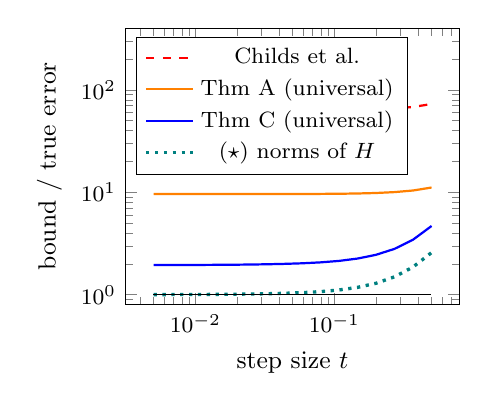
\begin{tikzpicture}
\begin{loglogaxis}[width=0.48\textwidth,height=0.42\textwidth,xlabel={step size $t$},
 ylabel={bound / true error},legend pos=north west,legend style={font=\footnotesize},
 tick label style={font=\footnotesize},label style={font=\small},ymin=0.8,ymax=400]
\addplot[red,dashed,thick] coordinates {(0.005012,62.86) (0.006813,62.86) (0.009261,62.86) (0.01259,62.87) (0.01711,62.87) (0.02326,62.88) (0.03162,62.9) (0.04299,62.93) (0.05843,62.99) (0.07943,63.1) (0.108,63.31) (0.1468,63.69) (0.1995,64.39) (0.2712,65.69) (0.3687,68.14) (0.5012,72.79)};
\addlegendentry{Childs et al.}
\addplot[orange,thick] coordinates {(0.005012,9.617) (0.006813,9.617) (0.009261,9.617) (0.01259,9.618) (0.01711,9.618) (0.02326,9.62) (0.03162,9.622) (0.04299,9.627) (0.05843,9.637) (0.07943,9.654) (0.108,9.685) (0.1468,9.743) (0.1995,9.85) (0.2712,10.05) (0.3687,10.42) (0.5012,11.14)};
\addlegendentry{Thm A (universal)}
\addplot[blue,thick] coordinates {(0.005012,1.95) (0.006813,1.951) (0.009261,1.954) (0.01259,1.958) (0.01711,1.963) (0.02326,1.971) (0.03162,1.983) (0.04299,2.001) (0.05843,2.028) (0.07943,2.071) (0.108,2.14) (0.1468,2.256) (0.1995,2.454) (0.2712,2.805) (0.3687,3.448) (0.5012,4.693)};
\addlegendentry{Thm C (universal)}
\addplot[teal,dotted,very thick] coordinates {(0.005012,1.003) (0.006813,1.004) (0.009261,1.006) (0.01259,1.008) (0.01711,1.011) (0.02326,1.016) (0.03162,1.022) (0.04299,1.033) (0.05843,1.048) (0.07943,1.073) (0.108,1.113) (0.1468,1.18) (0.1995,1.294) (0.2712,1.496) (0.3687,1.866) (0.5012,2.582)};
\addlegendentry{($\star$) norms of $H$}
\addplot[black,thin,domain=0.005:0.5] {1};
\end{loglogaxis}
\end{tikzpicture}\hfill
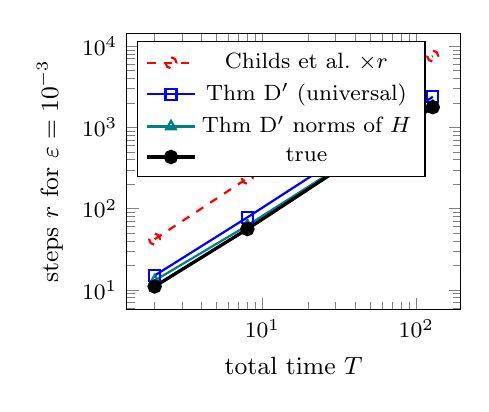
\begin{tikzpicture}
\begin{loglogaxis}[width=0.48\textwidth,height=0.42\textwidth,xlabel={total time $T$},
 ylabel={steps $r$ for $\varepsilon=10^{-3}$},legend pos=north west,legend style={font=\footnotesize},
 tick label style={font=\footnotesize},label style={font=\small}]
\addplot[red,dashed,thick,mark=o] coordinates {(2,42) (8,236) (32,1334) (128,7543)};
\addlegendentry{Childs et al.\ $\times r$}
\addplot[blue,thick,mark=square] coordinates {(2,15) (8,78) (32,426) (128,2380)};
\addlegendentry{Thm D$'$ (universal)}
\addplot[teal,thick,mark=triangle] coordinates {(2,13) (8,62) (32,330) (128,1815)};
\addlegendentry{Thm D$'$ norms of $H$}
\addplot[black,very thick,mark=*] coordinates {(2,11) (8,56) (32,314) (128,1776)};
\addlegendentry{true}
\end{loglogaxis}
\end{tikzpicture}
\caption{Transverse-field Ising chain $H=\sum_iZ_iZ_{i+1}+\sum_iX_i$, $n=8$ periodic, $A$ = $ZZ$ part,
$B$ = field part. \emph{Left:} one step, ratio of each rigorous bound to the true error
$\norm{S_4(t)-e^{-itH}}$ (computed exactly); the horizontal line is ratio~1. Childs et al.\ is
$\approx63\times$ the true error at small $t$, Theorem~A $\approx9.6\times$, Theorem~C (universal constants)
$\approx2\times$, and the operator-specific form \eqref{eq:star} tends to~1. \emph{Right:} Trotter steps needed
to reach error $10^{-3}$ at total time $T$; at $T=128$ the guarantee of Theorem~D$'$ with the norms of
$H$ is $1815$ against $1776$ truly needed ($+2.2\%$), while Childs et al.\ require $7543$.}
\label{fig:tfim}
\end{figure}

\paragraph{Prefactors on the Ising chain ($n=8$).} Evaluating each single-step bound with the
commutator norms of this $H$ ($\norm{E_5}=1.498$):
\begin{center}\small
\begin{tabular}{@{}ll@{}}
\toprule
bound & as a polynomial in $t$\\
\midrule
Childs et al.~\cite[(M13)]{Childs2021} & $94.17\,t^5$\\
Schubert--Mendl~\cite[Eq.~(9)]{SchubertMendl2023}, best split $s=6$ & $94.16\,t^5$\\
Theorem~A & $14.41\,t^5$\\
Theorem~B & $2.913\,t^5+10.12\,t^6$\\
Theorem~C & $2.913\,t^5+1.466\,t^6+9.648\,t^7$\\
exact leading term $\norm{E_5}$ (not a bound) & $1.498\,t^5$\\
\bottomrule
\end{tabular}
\end{center}
The Schubert--Mendl bound, evaluated with the actual operator norms of the nested stage commutators,
essentially reproduces the Childs et al.\ prefactor here; Theorem~A is $6.5\times$ smaller and the $t^5$
prefactor of Theorems~B and~C is $32\times$ smaller, within $1.95\times$ of the exact $\norm{E_5}$.

\paragraph{Error ratios across models.} For eight two-term models on $n=8$ qubits (TFIM at fields
$h\in\{0.2,0.5,1,2,5\}$, a mixed-field Ising chain, a Heisenberg chain and a random 2-local chain, the
last two split into even/odd bonds), at the step count that truly reaches $10^{-3}$ for $T=8$, the
ratio bound/true error is:
\begin{center}\small
\begin{tabular}{@{}lccc@{}}
\toprule
& worst-case error & error on $\lvert0\cdots0\rangle$ & error on a random state\\
\midrule
Childs et al.\ $\times r$ & $320$--$740$ & $360$--$1270$ & $750$--$1750$\\
Theorem D$'$, universal constants & $3.1$--$10.7$ & $4.6$--$25$ & $7.3$--$35$\\
Theorem D$'$, norms of $H$ & $1.5$--$6.5$ & $2.0$--$12$ & $3.6$--$17$\\
\bottomrule
\end{tabular}
\end{center}
Single step, Childs et al.\ is $31$--$116\times$ the true worst-case error, Theorem~C $1.4$--$4.5\times$,
and \eqref{eq:star} with the norms of $H$ $1.01$--$1.8\times$ ($t=0.01$--$0.1$). The remaining factor
$2$--$4$ between worst-case and typical-state errors cannot be closed by any operator-norm bound.

\paragraph{Large systems.} For open TFIM chains with $T=n$, $\varepsilon=10^{-3}$ (exact free-fermion
evaluation; true step counts computed exactly):
\begin{center}\small
\begin{tabular}{@{}rrrrrr@{}}
\toprule
$n$ & true & Thm D$'$ (norms of $H$) & Thm D$'$ (universal) & Thm C $\times r$ & Childs et al.\ $\times r$\\
\midrule
10 & 76 & 83 & 103 & 134 & 317\\
100 & 2449 & 2476 & 3224 & 4304 & 10266\\
300 & 12754 & 12824 & 16746 & 22377 & 53434\\
1000 & 77678 & 77966 ($+0.37\%$) & 101914 & 136160 & 325382\\
\bottomrule
\end{tabular}
\end{center}
The error bound of Childs et al.\ is $\ge300\times$ the true error at every size; the excess of
Theorem~D$'$ with the norms of $H$ shrinks from $9\%$ to $0.37\%$.

%======================================================================
\section{Verification and use of computer algebra}\label{sec:verification}

\paragraph{Exact arithmetic.} All Lie-polynomial computations (\code{trotter/}) use exact arithmetic in
$\Qc$ (elements $a_0+a_1\varpi+a_2\varpi^2$, $\varpi^3=2$, rational $a_i$; signs decided by rational
enclosures of $2^{1/3}$). Remainder integrals are bounded by rational interval Horner evaluation on 256
cells. Every inequality is additionally tested against exact matrix powers on random matrices
(\code{tests/}, 17 tests).

\paragraph{Alkahest CAS.} As an independent derivation of Proposition~\ref{prop:leading} that shares no
code with our own algebra, \code{trotter/alkahest\_bch.py} uses the Alkahest computer-algebra system
(v3.14)~\cite{Alkahest}. It declares noncommutative symbols $A,B$ and a commutative symbol $p$, builds the eleven
truncated exponentials and their product with Alkahest's noncommutative expansion
(\code{nc\_expand}/\code{nc\_terms}), truncating by degree after each multiplication (the untruncated
product exceeds Alkahest's term limits), and forms the truncated logarithm. It then substitutes
$p=1/(4-2^{2/3})$ and lets Alkahest's radical simplifier decide each claimed identity: degrees 1--4, and
all 32 degree-5 word coefficients against $\sum_ic_iC_i$ built with \code{alkahest.commutator}. All
identities hold; a tampered coefficient is rejected. Alkahest's ball arithmetic (\code{interval\_eval})
also confirms that each published decimal is an upper bound of its exact value. Using Alkahest exposed
features we had to supply ourselves (degree-truncated noncommutative products, BCH/logarithm of
products, Hall/Lyndon projection), which are natural additions to the system.

\paragraph{Lean kernel certificate.} \code{S4Leading.lean} (part of the same Lean project; uses only Lean core)
implements gcd-normalised rationals, $\Qc$ and truncated noncommutative series, recomputes $S_4$ and its
logarithm from $p$ alone, and proves by kernel evaluation (\code{decide}) that degrees 1--5 are as in
Proposition~\ref{prop:leading} and that both processing identities of Proposition~\ref{prop:Z} hold
(the slowest part of the build).

\paragraph{Lean/Mathlib formalisation.} \code{lean/TrotterAnalytic/} (Lean~v4.35.0~\cite{Lean4} + Mathlib~v4.35.0~\cite{Mathlib2020}, about 2100
lines, no \code{sorry}; \code{\#print axioms} shows only \code{propext}, \code{Classical.choice},
\code{Quot.sound}) proves, in any real Banach algebra with contraction-group generators:
Lemma~\ref{lem:voc} (variation of constants); Lemma~\ref{lem:tele} for every split, via the identity
$V_W(\mathrm{rev}(-L))=L^{-1}(W-V_L)L$; Lemma~\ref{lem:taylor} in chain form, using the integral form of
the conjugation remainder, obtained from a telescoping primitive without Fubini; the resulting
single-step theorem for any product formula and split; the telescoping and Euler--Maclaurin midpoint
lemmas; and Theorems~D and~D$'$ \emph{end to end}, with only the algebraic identities ($\hat c_r$,
$E_5=[H,Y]+Z$, $W_7=[H,Y_7]+Z_7$) as hypotheses. In a $C^*$-algebra all contraction hypotheses are
discharged for skew-adjoint generators, and the single-step theorem is instantiated for anti-Hermitian
complex matrices with the spectral norm. Not formalised: the identification of the abstract chain
coefficients with the computed Lie polynomials, and the interval bounds on the remainder integrals
(both done by exact arithmetic in Python).


\paragraph{Lean declarations relied on.} The project builds with Lean v4.35.0 and Mathlib v4.35.0
(\code{lake build}); \code{Axioms.lean} prints, for every declaration below, only the axioms
\code{propext}, \code{Classical.choice}, \code{Quot.sound}; there is no \code{sorry}, and no claim
relies on \code{native\_decide}. ``Lean-verified'' below means exactly this. Namespaces: \code{S4Cert}
(file \code{S4Leading.lean}) and \code{Trotter} (all other files).
{\small
\begin{longtable}{@{}>{\raggedright\arraybackslash}p{0.27\textwidth}>{\raggedright\arraybackslash}p{0.27\textwidth}>{\raggedright\arraybackslash}p{0.40\textwidth}@{}}
\toprule
Declaration & Claim supported & Difference between statement and claim\\
\midrule
\endhead
\code{S4Cert.p\_spec}, \code{degree1}, \dots, \code{degree5} & Proposition~\ref{prop:leading}, degrees 1--5 &
Stated for a computable model: truncated noncommutative polynomials (degree $\le5$) over an exact
implementation of $\Q[\varpi]/(\varpi^3-2)$, compared with a Boolean \code{polyEq}; not Mathlib's free
algebra. Vanishing of degree~6 (the $O(t^7)$) is checked in Python only.\\
\code{S4Cert.processing\_identity}, \code{processing\_identity\_A} & Proposition~\ref{prop:Z}: $E_5=[H,Y]+Z$ and
$E_5=[H,Y']+Z'$ & Same computable model as above.\\
\code{norm\_sub\_exp\_le\_integral}, \code{norm\_sub\_exp\_le\_integral\_split} & Lemma~\ref{lem:voc} &
Real Banach algebra; generators assumed to satisfy $\norm{e^{sa}}\le1$ (discharged in \code{CStar.lean}).\\
\code{hasDerivAt\_prodExp}, \code{chainV\_negrev}, \code{hasDerivAt\_split} & Lemma~\ref{lem:tele} &
Stages are an abstract list of generators $a_j$ (in the report $a_j=c_jX_j$).\\
\code{Ad\_sub\_taylor\_eq\_integral}, \code{norm\_chain\_sub\_taylor\_le\_grouped} & Lemma~\ref{lem:taylor} &
Chain coefficients and remainder constants are the abstract recursions \code{chainC}, \code{chainBg}.\\
\code{norm\_split\_sub\_exp\_le} & Inequality \eqref{eq:star} for every split $m$, hence the analytic
form of Theorems~\ref{thm:A}--\ref{thm:C} & The numerical constants of Theorems~A--C are \emph{not}
Lean-verified: identifying \code{chainC}/\code{chainBg} with the computed Lie polynomials and bounding
$\int_0^1\abs{c_{s,w}(u)}\dd u$ are done by exact and interval arithmetic in Python.\\
\code{norm\_split\_sub\_exp\_le\_skewAdjoint}, \code{matrix\_split\_sub\_exp\_le} & Applicability to
anti-Hermitian matrices & $C^*$-algebra / spectral-norm instance of the previous line.\\
\code{theoremD}, \code{singleStep\_input}, \code{theoremD\_full} & Theorem~\ref{thm:D} &
Hypotheses are the algebraic identities $\hat c_{0..3}=0$, $\hat c_4=5E_5$, $\hat c_5=-3[H,E_5]$,
$E_5=[H,Y]+Z$ and a bound $\norm{\hat S(\tau)-1}\le\beta$ on $[0,\delta]$ (the report takes $\beta=b(\delta)$);
the last term is $\norm{S-U}^2r(r-1)/2$, which is at most the report's $T^2b(\delta)^2/(2\delta^2)$.\\
\code{theoremDprime}, \code{singleStep\_input2}, \code{theoremDprime\_full} & Theorem~D$'$
(Appendix~\ref{app:proofs}) & As for Theorem~D, plus $\hat c_6$ and $W_7=[H,Y_7]+Z_7$ as hypotheses.\\
\bottomrule
\end{longtable}}
\noindent Not Lean-verified: the numerical values of all universal constants; Theorem~\ref{thm:E}
(proved in exact rational arithmetic in Python); Proposition~\ref{prop:struct}; and all numerics of
\S\ref{sec:numerics}. The problem has no official Lean statement; the statements above are ours.

%======================================================================
\section{Relation to prior work}\label{sec:prior}

\paragraph{Commutator-scaling bounds.} Childs and Su~\cite{ChildsSu2019} and Childs, Su, Tran, Wiebe and
Zhu~\cite{Childs2021} established bounds of the form $t^{p+1}\sum\gamma_w\norm{C_w}$ for order-$p$ formulas,
with explicit constants for two-term $S_4$ ($\sum\gamma_w=0.0875$). Schubert and
Mendl~\cite{SchubertMendl2023} generalise the construction with a free split point and report that for
fourth-order formulas the bounds still exceed the true error by about three orders of magnitude.
Their representation is that of Descombes and Thalhammer~\cite{DescombesThalhammer2010} (a split
variation-of-constants formula with integrated commutators); our Lemmas~\ref{lem:voc}--\ref{lem:tele}
are the same representation for bounded operators. The difference is in Lemma~\ref{lem:taylor}: we
expand from the right so that every surviving exponential is an outer unitary conjugation, and group
all terms sharing a conjugation, across Taylor orders, into one exact Lie polynomial before taking
norms. Recent work tightens bounds in other directions: ordering-aware bounds for geometrically local
lattice Hamiltonians~\cite{Liu2026}, which come close to exact fourth-order errors numerically;
Monte Carlo evaluation of commutator norms~\cite{Blunt2025}; explicit truncated BCH/Zassenhaus
constants~\cite{ArnalCasasRuizBenito2026}; and time-dependent and multi-product
formulas~\cite{ZhukRobertsonBravyi2024,AftabAnTrivisa2024,MizutaIkedaFujii2026,Mizuta2026,Bosse2025,WatsonWatkins2025}.
Our setting is complementary: generic bounded $A,B$ with operator-independent constants.

\paragraph{Leading-error coefficients.} That the leading local error is a Lie element and how to
generate order conditions in a Lie basis is standard~\cite{AuzingerHerfort2014,AKT2014,HLW2006}.
Leading-error coefficients of Suzuki- and Forest--Ruth-type schemes were tabulated numerically to optimise
schemes~\cite{McLachlan1995,Omelyan2002,Ostmeyer2023,Morales2025,MalezicOstmeyer2026}. In particular, Barthel
and Zhang~\cite{BarthelZhang2020} expanded exactly this $S_4$ in a Hall basis numerically and report the
measure $\varepsilon=(m/p)^p\sum_i\abs{c_i}\approx0.216883$ with $m=11$, $p=4$; this equals
$(11/4)^4\cdot0.0037922$, i.e.\ our $\sum_i\abs{c_i}$, a consistency check of Proposition~\ref{prop:leading}.
They also note that the coefficients depend on the Hall basis and minimise over the two orderings, a simple
form of our optimisation over representations. We are not aware of a previous closed form in $\Qc$, nor
of its use as the constant of a rigorous bound valid for all $t$.

\paragraph{Error cancellation over many steps.} Destructive interference of Trotter errors was proved for
first-order formulas by Tran et al.~\cite{Tran2020}, and Layden~\cite{Layden2022} related the first-order
error to a second-order formula. Y.-H.~Chen~\cite{ChenYH2025} separates, for general order, the
non-accumulating $[H,\cdot\,]$ component of the error, and B.~Chen, Xu, Yuan and Zhao~\cite{ChenXuYuanZhao2026}
show that interference occurs if and only if the leading error has this form. Theorems~D and~D$'$ are
therefore not a new mechanism; their contribution is a rigorous bound with every constant explicit for
$S_4$, the exact split $E_5=[H,Y]+Z$ with $\lb Z$ certified near-optimal, a second-order (degree-7 and
Euler--Maclaurin) refinement, and the processing interpretation~\cite{BlanesCasasRos1999}.

\paragraph{State- and structure-dependent bounds.} Much tighter error estimates are possible for
typical inputs, low-energy subspaces, locality or particle-number
structure~\cite{HeylHaukeZoller2019,Kivlichan2020,SuHuangCampbell2021,SahinogluSomma2021,ChenHKT2021,Zhao2022,YiCrosson2022,ChenBrandao2024,Burgarth2024,ZhaoZhouChilds2025}.
These are outside the operator-norm, commutator-form setting of the problem; our numerics quantify the
remaining factor $2$--$4$ between worst-case and typical-state errors.

\paragraph{Formal verification.} We know of no prior machine-checked proof of a higher-order product
formula error bound. The closest work verifies a first-order Trotter circuit in Lean with the error bound
as a precondition~\cite{QEDIA2026}; Mathlib provides Lie-algebra infrastructure~\cite{Nash2021,Mathlib2020}.
Our development uses Lean~4~\cite{Lean4} and Mathlib.

\paragraph{Other formulas.} Forest--Ruth/Yoshida~\cite{ForestRuth1990,Yoshida1990} and Suzuki's fractal
construction~\cite{Suzuki1990,Suzuki1991} are compared in Proposition~\ref{prop:struct}.

%======================================================================
\section{Limitations and next steps}\label{sec:limits}

\begin{itemize}[leftmargin=*]
\item \emph{Scope of formal verification.} The analytic argument is formal; the values of the
 constants rest on exact and interval arithmetic in Python (the leading term and processing identities
 are also kernel-checked). Connecting the two (evaluating the free-algebra identities in Mathlib) is the
 natural next step.
\item \emph{Optimality beyond the leading term.} Only the $t^5$ constant is proved optimal. For
 single-term all-$t$ bounds the gap between Theorem~A and our (non-exact) lower bound is $4.6\times$; for
 the secular constant it is $2.65\times$, and our $\lb Z$ is already optimal for bounds on $\norm Z$.
\item \emph{Worst case versus typical states.} Operator-norm bounds cannot capture the additional factor
 $2$--$4$ to the error on typical input states.
\item \emph{Two bounded summands.} We treat $H=A+B$ with bounded $A,B$. More summands, unbounded
 operators~\cite{DescombesThalhammer2010}, and other formulas (Proposition~\ref{prop:struct}) are natural
 extensions; the machinery is algorithmic in (formula, split, order).
\item \emph{Operator-specific numbers} (``norms of $H$'') use floating-point norms and a heuristic
 (Nelder--Mead) choice of $Y$; any $Y$ gives a valid bound.
\end{itemize}

\section*{AI disclosure}
This work was carried out with substantial assistance from Claude Opus~5.5. The AI wrote and ran the exact-arithmetic and numerical code, the Lean formalisation, the
linear-programming certificates and drafts of this report, under the direction of the author, who
chose the problem, set the goals and reviewed the results. All claims are backed by code in the
accompanying repository; rigorous claims are machine-checked or computer-assisted as described in
\S\ref{sec:verification}.

%======================================================================
\begin{appendices}
\section{Proofs}\label{app:proofs}

\begin{proof}[Proof of Lemma~\ref{lem:voc}]
Differentiating $S_4=LR$,
\[
S_4'-HS_4=L'R+LR'-HLR=L\bigl(L^{-1}L'+R'R^{-1}-L^{-1}HL\bigr)R .
\]
Then
\[
\frac{d}{d\tau}\bigl[U(-\tau)S_4(\tau)\bigr]=U(-\tau)\bigl(S_4'-HS_4\bigr);
\]
integrate from $0$ to $t$ and use that $U$, $L$, $R$ are unitary.
\end{proof}

\begin{proof}[Proof of Lemma~\ref{lem:tele}]
For a product $P(\tau)=\prod_je^{\tau a_j}$, with $P_j$ the product of the first $j-1$ factors,
\[
P'=\sum_jP_ja_jP_j^{-1}\,P,\qquad \sum_jP_ja_jP_j^{-1}=V(\tau)\quad(\text{terminal }0).
\]
For the left factor one checks by induction on $L$ that the reversed, negated chain with terminal $W$
satisfies
\[
V_W(\mathrm{rev}(-L))=L^{-1}(W-V_L)L;
\]
with $W=H$ this gives $L^{-1}L'-L^{-1}HL=-V_{\rm left}$.
\end{proof}

\begin{proof}[Proof of Lemma~\ref{lem:taylor}]
For a single conjugation,
\[\Phi(\sigma)=\sum_{i\le k}\frac{(\tau-\sigma)^i}{i!}\Ad_{e^{\sigma a}}(\ad_a^iX)\]
has derivative (the sum telescopes)
\[
\Phi'(\sigma)=\frac{(\tau-\sigma)^k}{k!}\Ad_{e^{\sigma a}}(\ad_a^{k+1}X),
\]
so
\[
\Ad_{e^{\tau a}}X-\sum_{i\le k}\frac{\tau^i}{i!}\ad_a^iX=\int_0^\tau\frac{(\tau-\sigma)^k}{k!}
\Ad_{e^{\sigma a}}(\ad_a^{k+1}X)\dd\sigma .
\]
For a chain $a{:}L$, write
\[
V_{a:L}=a+\Ad_{e^{\tau a}}\Bigl(E_L+\sum_{j<K}\tau^jc(L,j)\Bigr),
\]
with $E_L$ the remainder of $L$. Expanding each
$\Ad_{e^{\tau a}}c(L,j)$ to order $K-j$ reproduces the recursion for $c(a{:}L,\cdot)$ (a reindexing of
a double sum), leaves $\Ad_{e^{\tau a}}E_L$, of norm $\norm{E_L}$, and leaves
\[\int_0^\tau\Ad_{e^{\sigma a}}\Bigl(\sum_j\tau^j\frac{(\tau-\sigma)^{K-j-1}}{(K-j-1)!}\ad_a^{K-j}c(L,j)\Bigr)\dd\sigma,\]
whose norm is at most the integral of the norm of the bracket; substituting $\sigma=\tau u$ gives the
item's term $\tau^K\int_0^1\norm{P(u)}\dd u$. Induction over the chain finishes the proof.
\end{proof}

\begin{proof}[Proof of Theorem~\ref{thm:D}]
\emph{Step 1.} The identity $S^r-U^r=\sum_{j<r}U^{r-1-j}(S-U)S^j$ gives
\[
\Bigl\lVert S^r-U^r-\sum_jU^{r-1-j}(S-U)U^j\Bigr\rVert\le\norm{S-U}^2\,\frac{r(r-1)}2,
\qquad U^{r-1-j}(S-U)U^j=U^r\Ad_{U(-j\delta)}M .
\]
\emph{Step 2.} By Lemma~\ref{lem:tele} with first generator $-H$, $\hat S'=\hat V\hat S$, so
$M=\int_0^\delta\hat V\hat S$. Lemma~\ref{lem:taylor} with $\hat c_0=\dots=\hat c_3=0$, $\hat c_4=5E_5$,
$\hat c_5=-3[H,E_5]$, and the $K=2$ conjugation remainder of $\Ad_{U(-\delta/2)}E_5$, give
\[
\norm{M-\delta^5\Ad_{U(-\delta/2)}E_5}\le\frac{\delta^7\hat\Gamma_7}7+\frac{\delta^7\norm{\ad_H^2E_5}}8
+\hat\Gamma_5\int_0^\delta\tau^4b(\tau)\dd\tau .
\]
\emph{Step 3.} With $f(s)=\Ad_{U(-s)}Y$ and midpoints $m_j=(j+\frac12)\delta$, the $K=2$ remainder at
$\pm u$ gives for each cell
\[
\norm{f((j{+}1)\delta)-f(j\delta)+\delta\,\Ad_{U(-m_j)}[H,Y]}\le\frac{\delta^3}{24}\norm{\ad_H^3Y},
\]
and $\sum_j\bigl[f((j{+}1)\delta)-f(j\delta)\bigr]=f(T)-f(0)$ has norm at most $2\norm Y$.
Collecting the terms with $E_5=[H,Y]+Z$ gives the statement.
\end{proof}

\paragraph{Theorem D$'$.} Under the hypotheses of Theorem~D, let
\[
W_7=\frac{\hat c_6}7-\frac{\ad_H^2E_5}8=[H,Y_7]+Z_7,\qquad c_5=\frac1{576}+\frac1{1920}.
\]
Then
\[
\begin{aligned}
\norm{S_4(\delta)^r-e^{TH}}\le{}&T\delta^4\norm Z+2\delta^4\norm Y+\delta^6\tfrac{\norm{\ad_H^2Y}}{12}
+T\delta^8c_5\norm{\ad_H^5Y}\\&+T\delta^6\norm{Z_7}+2\delta^6\norm{Y_7}+T\delta^8\tfrac{\norm{\ad_H^3Y_7}}{24}\\
&+T\delta^7\Bigl(\tfrac{\hat\Gamma_8}8+\tfrac{\norm{\ad_H^3E_5}}{48}+\tfrac{\norm{[H,W_7]}}2\Bigr)
+T\delta^4\hat\Gamma_5\tfrac{b(\delta)}5+\tfrac{T^2b(\delta)^2}{2\delta^2}.
\end{aligned}
\]
The proof adds the exact degree-7 term to Step~2, telescopes $W_7$ like $E_5$, and replaces the midpoint
estimate by the Euler--Maclaurin version, with cell error
\[
\frac{(2h)^5}{1920}\norm{\ad^5Y}
\]
(from the $K=4$ remainder at $\pm u$, with the $\delta^3/24$ correction telescoped again). The universal
constants are
\[
\begin{gathered}
\lb{Z_7}=0.0001192,\quad \lb{Y_7}=0.00003441,\quad \tfrac{\lb{\ad_H^2Y}}{12}=0.0003512,\quad
c_5\lb{\ad_H^5Y}=0.0000761,\\
\tfrac{\lb{\hat\Gamma_8}}{8}=0.001328,\quad \tfrac{\lb{\ad_H^3E_5}}{48}=0.0004997,\quad
\tfrac{\lb{[H,W_7]}}{2}=0.0001362 .
\end{gathered}
\]

\section{Constant tables}\label{app:tables}

\begin{table}[ht]
\centering\small
\caption{Leading term over right-nested commutators: $E_5=-\sum_w\epsilon_w\C w$ with $\epsilon_w>0$.
$\C{ABA}=\C{AAB}$ and $\C{BBA}=\C{BAB}$ do not appear.}\label{tab:E5}
\begin{tabular}{@{}lll@{}}
\toprule
$\C w$ & $\epsilon_w\in\Qc$ & $\le$\\
\midrule
$\C{AAA}$ & $\tfrac{169}{1350000}+\tfrac{1}{28125}\varpi+\tfrac{2437}{43200000}\varpi^2$ & 0.0002596\\
$\C{AAB}$ & $\tfrac{301}{900000}+\tfrac{67}{900000}\varpi+\tfrac{59}{400000}\varpi^2$ & 0.0006624\\
$\C{ABB}$ & $\tfrac{17}{150000}-\tfrac{49}{1350000}\varpi+\tfrac{109}{2700000}\varpi^2$ & 0.0001317\\
$\C{BAA}$ & $\tfrac{449}{2700000}+\tfrac{61}{900000}\varpi+\tfrac{211}{2700000}\varpi^2$ & 0.0003758\\
$\C{BAB}$ & $\tfrac{449}{900000}+\tfrac{61}{300000}\varpi+\tfrac{211}{900000}\varpi^2$ & 0.0011273\\
$\C{BBB}$ & $\tfrac{301}{1350000}+\tfrac{67}{1350000}\varpi+\tfrac{59}{600000}\varpi^2$ & 0.0004416\\
\midrule
$\sum$ & & 0.0029984\\
\bottomrule
\end{tabular}
\end{table}

\paragraph{Comparison with Childs et al.} Proposition J.1 (Eq.~(M13)) of~\cite{Childs2021} bounds the
error by
\[
t^5\sum_w\gamma_w\norm{[X_1,[X_2,[X_3,[B,A]]]]},
\]
and these norms equal $\norm{\C w}$ for $w=X_1X_2X_3$. Their coefficients and those of Theorem~A are
listed below.
\begin{center}\small
\begin{tabular}{@{}lcc@{}}
\toprule
$w$ & \cite{Childs2021} & Theorem~A\\
\midrule
$\mathsf{AAA}$ & 0.0047 & 0.000675\\
$\mathsf{AAB}$ & 0.0057 & 0.002040\\
$\mathsf{ABA}$ & 0.0046 & 0\\
$\mathsf{ABB}$ & 0.0074 & 0.001668\\
$\mathsf{BAA}$ & 0.0097 & 0.001424\\
$\mathsf{BAB}$ & 0.0097 & 0.004279\\
$\mathsf{BBA}$ & 0.0173 & 0\\
$\mathsf{BBB}$ & 0.0284 & 0.003583\\
\midrule
$\sum$ & 0.0875 & 0.01367\\
\bottomrule
\end{tabular}
\end{center}
The per-commutator constants of Theorems~B and~C (10 and 24 nonzero coefficients for the $t^6$ and $t^7$
remainders) and of Theorems~D,~D$'$ are listed in \code{results/constants.md} of the repository.

%======================================================================
\end{appendices}

\begin{thebibliography}{99}
\small
\bibitem{Childs2021} A.~M. Childs, Y.~Su, M.~C. Tran, N.~Wiebe, and S.~Zhu, Theory of Trotter error with commutator scaling, \emph{Phys. Rev. X} \textbf{11}, 011020 (2021), doi:10.1103/PhysRevX.11.011020, arXiv:1912.08854.
\bibitem{ChildsSu2019} A.~M. Childs and Y.~Su, Nearly optimal lattice simulation by product formulas, \emph{Phys. Rev. Lett.} \textbf{123}, 050503 (2019), doi:10.1103/PhysRevLett.123.050503, arXiv:1901.00564.
\bibitem{SchubertMendl2023} A.~Schubert and C.~B. Mendl, Trotter error with commutator scaling for the Fermi--Hubbard model, \emph{Phys. Rev. B} \textbf{108}, 195105 (2023), doi:10.1103/PhysRevB.108.195105, arXiv:2306.10603.
\bibitem{DescombesThalhammer2010} S.~Descombes and M.~Thalhammer, An exact local error representation of exponential operator splitting methods for evolutionary problems and applications to linear Schr\"odinger equations in the semi-classical regime, \emph{BIT Numer. Math.} \textbf{50}, 729--749 (2010), doi:10.1007/s10543-010-0282-4.
\bibitem{AuzingerHerfort2014} W.~Auzinger and W.~Herfort, Local error structures and order conditions in terms of Lie elements for exponential splitting schemes, \emph{Opuscula Math.} \textbf{34}(2), 243--255 (2014), doi:10.7494/OpMath.2014.34.2.243.
\bibitem{AKT2014} W.~Auzinger, O.~Koch, and M.~Thalhammer, Defect-based local error estimators for splitting methods, with application to Schr\"odinger equations, Part~II: Higher-order methods for linear problems, \emph{J. Comput. Appl. Math.} \textbf{255}, 384--403 (2014), doi:10.1016/j.cam.2013.04.043.
\bibitem{Layden2022} D.~Layden, First-order Trotter error from a second-order perspective, \emph{Phys. Rev. Lett.} \textbf{128}, 210501 (2022), doi:10.1103/PhysRevLett.128.210501, arXiv:2107.08032.
\bibitem{Suzuki1990} M.~Suzuki, Fractal decomposition of exponential operators with applications to many-body theories and Monte Carlo simulations, \emph{Phys. Lett. A} \textbf{146}, 319--323 (1990), doi:10.1016/0375-9601(90)90962-N.
\bibitem{Suzuki1991} M.~Suzuki, General theory of fractal path integrals with applications to many-body theories and statistical physics, \emph{J. Math. Phys.} \textbf{32}, 400--407 (1991), doi:10.1063/1.529425.
\bibitem{Yoshida1990} H.~Yoshida, Construction of higher order symplectic integrators, \emph{Phys. Lett. A} \textbf{150}, 262--268 (1990), doi:10.1016/0375-9601(90)90092-3.
\bibitem{ForestRuth1990} E.~Forest and R.~D. Ruth, Fourth-order symplectic integration, \emph{Physica D} \textbf{43}, 105--117 (1990), doi:10.1016/0167-2789(90)90019-L.
\bibitem{BlanesCasasRos1999} S.~Blanes, F.~Casas, and J.~Ros, Symplectic integration with processing: a general study, \emph{SIAM J. Sci. Comput.} \textbf{21}, 711--727 (1999), doi:10.1137/S1064827598332497.
\bibitem{HLW2006} E.~Hairer, C.~Lubich, and G.~Wanner, \emph{Geometric Numerical Integration: Structure-Preserving Algorithms for Ordinary Differential Equations}, 2nd ed., Springer Series in Computational Mathematics, Vol.~31 (Springer, Berlin, 2006), doi:10.1007/3-540-30666-8.
\bibitem{McLachlan1995} R.~I. McLachlan, On the numerical integration of ordinary differential equations by symmetric composition methods, \emph{SIAM J. Sci. Comput.} \textbf{16}, 151--168 (1995), doi:10.1137/0916010.
\bibitem{Omelyan2002} I.~P. Omelyan, I.~M. Mryglod, and R.~Folk, Optimized Forest--Ruth- and Suzuki-like algorithms for integration of motion in many-body systems, \emph{Comput. Phys. Commun.} \textbf{146}, 188--202 (2002), doi:10.1016/S0010-4655(02)00451-4.
\bibitem{BarthelZhang2020} T.~Barthel and Y.~Zhang, Optimized Lie--Trotter--Suzuki decompositions for two and three non-commuting terms, \emph{Ann. Phys.} \textbf{418}, 168165 (2020), doi:10.1016/j.aop.2020.168165, arXiv:1901.04974.
\bibitem{Ostmeyer2023} J.~Ostmeyer, Optimised Trotter decompositions for classical and quantum computing, \emph{J. Phys. A: Math. Theor.} \textbf{56}, 285303 (2023), doi:10.1088/1751-8121/acde7a, arXiv:2211.02691.
\bibitem{MalezicOstmeyer2026} M.~Male\v{z}i\v{c} and J.~Ostmeyer, Efficient Trotter--Suzuki schemes for long-time quantum dynamics, \emph{J. Phys. A: Math. Theor.} \textbf{59}, 345301 (2026), doi:10.1088/1751-8121/ae919f, arXiv:2601.18756.
\bibitem{Morales2025} M.~E.~S. Morales, P.~C.~S. Costa, G.~Pantaleoni, D.~K. Burgarth, Y.~R. Sanders, and D.~W. Berry, Selection and improvement of product formulae for best performance of quantum simulation, \emph{Quantum Inf. Comput.} \textbf{25}(1), 1--35 (2025), doi:10.2478/qic-2025-0001, arXiv:2210.15817.
\bibitem{Tran2020} M.~C. Tran, S.-K. Chu, Y.~Su, A.~M. Childs, and A.~V. Gorshkov, Destructive error interference in product-formula lattice simulation, \emph{Phys. Rev. Lett.} \textbf{124}, 220502 (2020), doi:10.1103/PhysRevLett.124.220502, arXiv:1912.11047.
\bibitem{ChenYH2025} Y.-H. Chen, Trotter error time scaling separation via commutant decomposition, \emph{Phys. Rev. A} \textbf{111}, 022612 (2025), doi:10.1103/PhysRevA.111.022612, arXiv:2409.16634.
\bibitem{ChenXuYuanZhao2026} B.~Chen, J.~Xu, X.~Yuan, and Q.~Zhao, General framework for error interference in quantum simulation, \emph{Phys. Rev. Lett.} \textbf{136}, 200601 (2026), doi:10.1103/g2n5-qdxh, arXiv:2411.03255.
\bibitem{SuHuangCampbell2021} Y.~Su, H.-Y. Huang, and E.~T. Campbell, Nearly tight Trotterization of interacting electrons, \emph{Quantum} \textbf{5}, 495 (2021), doi:10.22331/q-2021-07-05-495, arXiv:2012.09194.
\bibitem{HeylHaukeZoller2019} M.~Heyl, P.~Hauke, and P.~Zoller, Quantum localization bounds Trotter errors in digital quantum simulation, \emph{Sci. Adv.} \textbf{5}, eaau8342 (2019), doi:10.1126/sciadv.aau8342, arXiv:1806.11123.
\bibitem{Kivlichan2020} I.~D. Kivlichan, C.~Gidney, D.~W. Berry, N.~Wiebe, J.~McClean, W.~Sun, Z.~Jiang, N.~Rubin, A.~Fowler, A.~Aspuru-Guzik, H.~Neven, and R.~Babbush, Improved fault-tolerant quantum simulation of condensed-phase correlated electrons via Trotterization, \emph{Quantum} \textbf{4}, 296 (2020), doi:10.22331/q-2020-07-16-296, arXiv:1902.10673.
\bibitem{SahinogluSomma2021} B.~\c{S}ahino\u{g}lu and R.~D. Somma, Hamiltonian simulation in the low-energy subspace, \emph{npj Quantum Inf.} \textbf{7}, 119 (2021), doi:10.1038/s41534-021-00451-w, arXiv:2006.02660.
\bibitem{ChenHKT2021} C.-F. Chen, H.-Y. Huang, R.~Kueng, and J.~A. Tropp, Concentration for random product formulas, \emph{PRX Quantum} \textbf{2}, 040305 (2021), doi:10.1103/PRXQuantum.2.040305, arXiv:2008.11751.
\bibitem{ChenBrandao2024} C.-F. Chen and F.~G.~S.~L. Brand\~ao, Average-case speedup for product formulas, \emph{Commun. Math. Phys.} \textbf{405}, 32 (2024), doi:10.1007/s00220-023-04912-5, arXiv:2111.05324.
\bibitem{Zhao2022} Q.~Zhao, Y.~Zhou, A.~F. Shaw, T.~Li, and A.~M. Childs, Hamiltonian simulation with random inputs, \emph{Phys. Rev. Lett.} \textbf{129}, 270502 (2022), doi:10.1103/PhysRevLett.129.270502, arXiv:2111.04773.
\bibitem{ZhaoZhouChilds2025} Q.~Zhao, Y.~Zhou, and A.~M. Childs, Entanglement accelerates quantum simulation, \emph{Nat. Phys.} \textbf{21}, 1338--1345 (2025), doi:10.1038/s41567-025-02945-2, arXiv:2406.02379.
\bibitem{YiCrosson2022} C.~Yi and E.~Crosson, Spectral analysis of product formulas for quantum simulation, \emph{npj Quantum Inf.} \textbf{8}, 37 (2022), doi:10.1038/s41534-022-00548-w, arXiv:2102.12655.
\bibitem{Burgarth2024} D.~Burgarth, P.~Facchi, A.~Hahn, M.~Johnsson, and K.~Yuasa, Strong error bounds for Trotter and Strang-splittings and their implications for quantum chemistry, \emph{Phys. Rev. Research} \textbf{6}, 043155 (2024), doi:10.1103/PhysRevResearch.6.043155, arXiv:2312.08044.
\bibitem{ZhukRobertsonBravyi2024} S.~Zhuk, N.~F. Robertson, and S.~Bravyi, Trotter error bounds and dynamic multi-product formulas for Hamiltonian simulation, \emph{Phys. Rev. Research} \textbf{6}, 033309 (2024), doi:10.1103/PhysRevResearch.6.033309, arXiv:2306.12569.
\bibitem{MizutaIkedaFujii2026} K.~Mizuta, T.~N. Ikeda, and K.~Fujii, Theory of Trotter errors for time-dependent product and multi-product formulas, \emph{PRX Quantum} \textbf{7}, 033061 (2026), doi:10.1103/ywv1-7fhf, arXiv:2410.14243.
\bibitem{Mizuta2026} K.~Mizuta, On the commutator scaling in Hamiltonian simulation with multi-product formulas, \emph{Quantum} \textbf{10}, 1974 (2026), doi:10.22331/q-2026-01-19-1974, arXiv:2507.06557.
\bibitem{AftabAnTrivisa2024} J.~Aftab, D.~An, and K.~Trivisa, Multi-product Hamiltonian simulation with explicit commutator scaling, arXiv:2403.08922 (2024).
\bibitem{WatsonWatkins2025} J.~D. Watson and J.~Watkins, Exponentially reduced circuit depths using Trotter error mitigation, \emph{PRX Quantum} \textbf{6}, 030325 (2025), doi:10.1103/kw39-yxq5, arXiv:2408.14385.
\bibitem{Bosse2025} J.~L. Bosse, A.~M. Childs, C.~Derby, F.~M. Gambetta, A.~Montanaro, and R.~A. Santos, Efficient and practical Hamiltonian simulation from time-dependent product formulas, \emph{Nat. Commun.} \textbf{16}, 2673 (2025), doi:10.1038/s41467-025-57580-5.
\bibitem{Liu2026} Z.~Liu, Z.-Y. Wei, M.~Foss-Feig, A.~V. Gorshkov, and A.~M. Childs, Ordering-aware theory of Trotter error, arXiv:2610.03672 (2026).
\bibitem{ArnalCasasRuizBenito2026} A.~Arnal, F.~Casas, and J.~L. Ruiz-Benito, Error bounds for the truncated Baker--Campbell--Hausdorff and Zassenhaus formulas in unitary problems, arXiv:2607.07692 (2026).
\bibitem{Blunt2025} N.~S. Blunt, A.~V. Ivanov, and A.~J. Bay-Smidt, A Monte Carlo approach to bound Trotter error, arXiv:2510.11621 (2025).
\bibitem{QEDIA2026} Y.~Ren, Z.~Zhang, J.~Liu, J.~Li, Y.~Qi, and M.~Ying, QEDIA: Quantum program verification in Lean, arXiv:2610.17708 (2026).
\bibitem{Nash2021} O.~Nash, Formalising Lie algebras, arXiv:2112.04570 (2021).
\bibitem{Hall1950} M.~Hall, A basis for free Lie rings and higher commutators in free groups,
\emph{Proc.\ Amer.\ Math.\ Soc.} \textbf{1}, 575--581 (1950).
\bibitem{Reutenauer1993} C.~Reutenauer, \emph{Free Lie Algebras}, London Mathematical Society Monographs,
New Series, Vol.~7 (Oxford University Press, 1993).
\bibitem{Alkahest} Alkahest Contributors, \emph{Alkahest: a high-performance computer algebra system for
Python}, version 3.14.0 (2026), \url{https://github.com/alkahest-cas/alkahest}.
\bibitem{Lean4} L.~de Moura and S.~Ullrich, The Lean 4 theorem prover and programming language, in
\emph{Automated Deduction -- CADE 28}, LNCS \textbf{12699}, 625--635 (Springer, 2021).
\bibitem{Mathlib2020} The mathlib Community, The Lean mathematical library, in \emph{Proc.\ 9th ACM SIGPLAN
Int.\ Conf.\ on Certified Programs and Proofs (CPP 2020)}, 367--381 (ACM, 2020).
\end{thebibliography}

\end{document}
